%ब 
\section{Baseline Experiment} \label{s:results-Baseline}

The performance of Cassandra when referential
integrity validations are introduced  is compared with
 a baseline experiment where the operations on the entities do not trigger any
such validations.  Such a baseline serves as a reference to determine the
difference in performance of the \ac{DBMS} when validations are imposed using
the \ac{API} and to analyse the performance of the solutions. 

In the baseline experiment,  the operations on the entities represent how
operations on data are performed in Cassandra without referential integrity
validations. In order to be consistent with the solutions, the operations
\texttt{Create}, \texttt{Update} and \texttt{Delete} for the baseline are
measured in the same way it is measured for the solutions and the artificial
data for the baseline experiment is created the same way as well.
Note that, \texttt{Create} inserts all the entities for \texttt{Student},
\texttt{Course} and \texttt{Enrolment}.  \texttt{Update} performs changes on the
primary keys of \texttt{Student} and \texttt{Course} entities,  and on the
foreign keys (\texttt{CourseId}) of \texttt{Enrolment} while \texttt{Delete}
removes all the \texttt{Student},  \texttt{Course} and \texttt{Enrolment}
entities. These operations are performed precisely the same way as the
solutions, so that the comparison and analysis of results are balanced and
unbiased.

The results in terms of average response time and throughput for the baseline
experiment are presented as  bar-plots in Figure~\ref{fres:Baseline}. 
Specifically,  Figure~\ref{fres:Baseline-responsetime} shows the response time 
of each operation on a single entity in the three column families. 
Figure~\ref{fres:Baseline-throughput} presents the throughput of each operation
on the three column families in one second. 
% The analysis of the performance of each operation on an entity is discussed as
% follows. 

% 	\begin{figure}[h] \centering
% 	\includegraphics[width=. 8\textwidth]{. /figure/result/barplot-Baseline-rt.pdf}
% 		\caption{Baseline}\label{fr:Solution0-barplot}
% 	\end{figure}
	
	\begin{figure}[H]
		
		\subfigure[Response time]
		{\includegraphics[width=\Width]{figure/result/barplot-Baseline-rt.pdf}\label{fres:Baseline-responsetime}}
		\subfigure[Throughput]
		{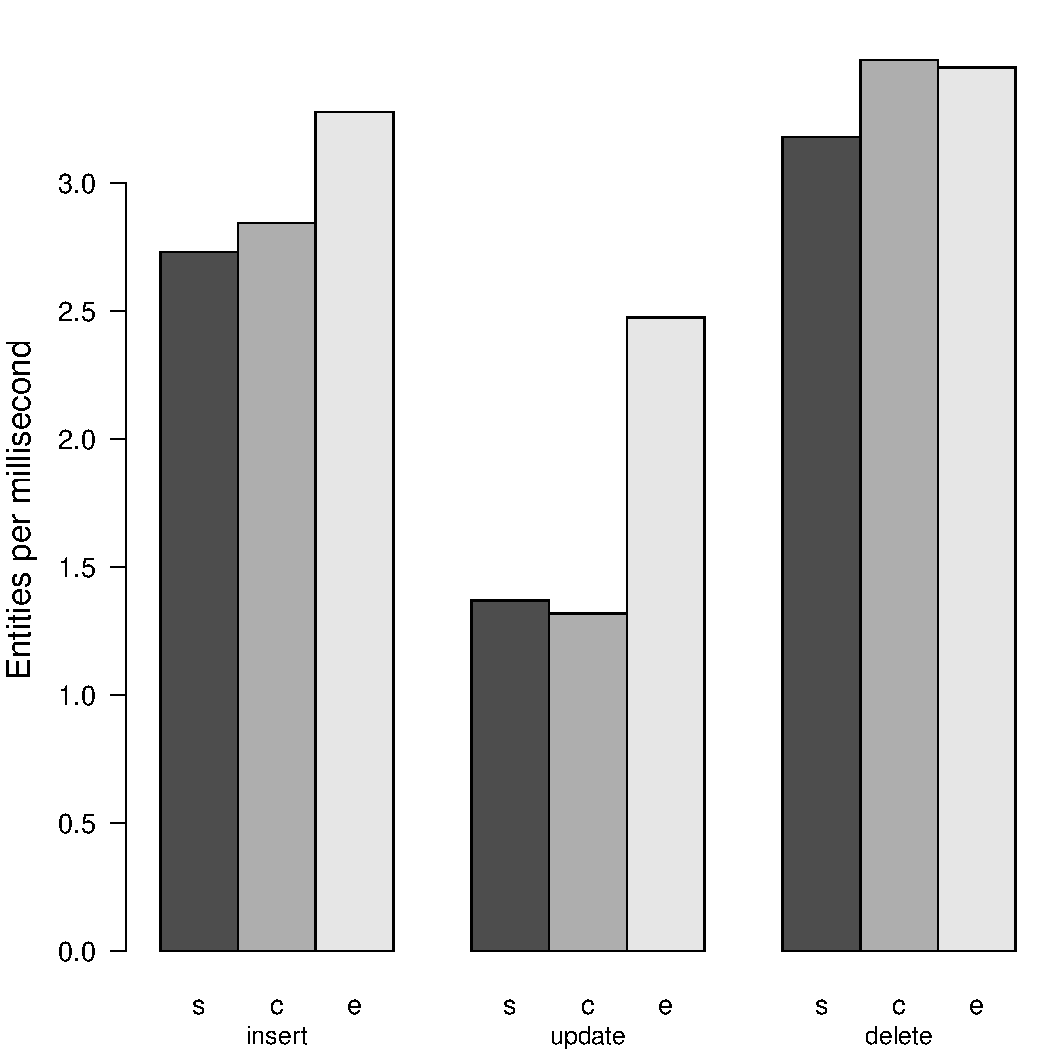
\includegraphics[width=\Width]{figure/result/barplot-Baseline-tp.pdf}\label{fres:Baseline-throughput}}
		\caption{Performance of Baseline}\label{fres:Baseline}
	\end{figure}

As seen from these results,  the \texttt{delete} operation takes in average the
least response time and  highest throughput,  respectively.  That is,  the time to
delete an entity is shorter when compared to \texttt{insert} or \texttt{update}, 
which also means that more \texttt{delete} operations can be performed within a
second.  On the other hand,  \texttt{update} takes the most time to complete all
the operations thus providing a smaller throughput while \texttt{insert} is
faster than \texttt{update} but takes slightly more time than \texttt{delete}. 

The \texttt{delete} operation performs faster than the other operations because
Cassandra performs  tombstone deletes,  where data is not physically but only
logically marked as deleted.  The \texttt{update} operation takes the most time
because it requires searching by index to access the correct columns in the
column family.  Moreover,   an \texttt{update} involves  \texttt{insert} and
\texttt{delete} operations hence takes more time that the \texttt{delete}
operation. Note that the \texttt{update} in \texttt{Enrolment} takes lesser time
because it does not change the primary keys of these entities and only the
foreign key attributes are changed.  % On the other hand,
% \texttt{update} on \texttt{Student} and \texttt{Course} entities changes the
% primary keys,  which involves performing an \texttt{insert} and a
% \texttt{delete} operation for each entity.
The \texttt{insert} operation takes slightly more time than \texttt{delete}
since data has to be physically written into the column families.

The time taken to insert one entity of \texttt{Student},  \texttt{Course} and
\texttt{Enrolment} are similar since there are no additional validations or
operations to insert these entities.  Note that the slight variations in the
perfromance for an \texttt{insert} on these entities can be due to
difference in columns,  size and external factors. 